\documentclass[../main]{subfiles}
\begin{document}

\section{Progettazione software}
La progettazione è l'attività che viene svolta prima della codifica e subito dopo l'analisi dei requisiti. Mentre l'analisi dei requisiti si occupa di \textit{cosa} è giusto fare, la progettazione si occupa di \textit{come} è giusto farlo.\newline
La progettazione deve essere fatta con un approccio \textit{divide et impera} per governare la complessità del prodotto, ripartendo le responsabilità per realizzare il prodotto con \g{efficienza} e con garantendo qualità (con \g{efficacia}).
\subsection{Dall'analisi alla progettazione}
Il primo step dell'attività di progettazione è accertarsi che il dominio e i requisiti da realizzare siano corretti, che i vincoli da rispettare siano soddisfatti. Subito dopo, prima di pensare al codice, va fissata l'architettura del prodotto.
\begin{figure}[h]
    \begin{center}
        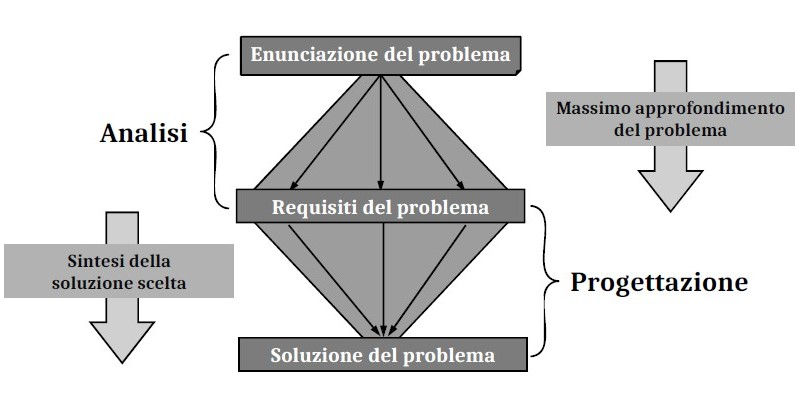
\includegraphics[scale=0.6]{immagini/progettazione.jpg}
    \end{center}
\end{figure}
\subsection{Obiettivi della progettazione}
Il progettista intende realizzare il proprio prodotto con obiettivi di qualità.\newline
Un'\g{architettura} si può definire di qualità se è:
\begin{itemize}
    \item Sufficiente: ha in sé tutto ciò che è necessario per soddisfare i requisiti;
    \item Comprensibile: deve essere compresa dagli stakeholder;
    \item Modulare: divisibile in blocchi componibili (parti chiare e ben distinte), coesi, che facilitino le modifiche, perseguendo l'information hiding;
    \item Robusto: capace di supportare input validi e/o non validi e comportarsi nel modo adatto di conseguenza.
    \item Flessibile: se variano i requisiti, le modifiche da effettuare sono contenute;
    \item Riusabile: le componenti create possono essere riusate in altri prodotti. Nel breve periodo questo risulta costoso, perché significa perdere più tempo anche in componenti che potrebbero non richiederlo, ma nel lungo periodo gli effetti del riuso fanno risparmiare parecchie risorse (è un investimento);
    \item \g{Efficiente}: nello spazio, nel tempo;
    \item Affidabile (\textit{reliable}): fa quello che dichiara e i comportamenti attesi (buon funzionamento) valgono anche in situazioni di errore;
    \item Disponibile (\textit{available}): funziona quando ne ho bisogno e se deve essere manutenuta è necessario interrompere solo una minima parte (il software non deve essere un monolite);
    \item Sicuro rispetto a malfunzionamenti (\textit{safe}): esente da malfunzionamenti gravi;
    \item Sicuro rispetto a intrusioni (\textit{secure}): dati e funzioni non sono vulnerabili a intrusioni;
\end{itemize}
\subsection{Progettazione modulare}
In particolare, l'architettura deve essere modulare ma ci devono essere poche dipendenze fra le componenti: l'obiettivo di una buona architettura è minimizzare le dipendenze \textit{"cattive"}. Un modulo può essere:
\begin{itemize}
    \item un'interfaccia: corrisponde a una porzione di codice che funziona come un "contratto d'uso" per il modulo. Tipicamente, da solo non permette il funzionamento di un'applicazione. Un modulo di tipo interfaccia è tipicamente la chiave d'ingresso a una serie di più funzionalità che raggiungono gli obiettivi dichiarati dall'interfaccia in modi diversi;
    \item un'implementazione: corrisponde a una porzione di codice che fornisce una funzionalità e dovrebbe, nella maggior parte dei casi, \textit{implementare} un'interfaccia. È rischioso far dipendere un modulo da un'implementazione, poiché una sua modifica potrebbe avere gravi conseguenze (catena di modifiche a cascata da fare).
\end{itemize}
\subsection{Ulteriori caratteristiche di qualità}
Altre caratteristiche che un'architettura deve avere:
\begin{itemize}
    \item Semplicità: ogni parte fa lo stretto necessario e non di più;
    \item \textit{Information hiding}: le dipendenze devono essere sulle interfacce e non sulle implementazioni, avendo come buone conseguenze la possibilità di un maggior riutilizzo e di un minor numero di dipendenze e che cambi di implementazioni non inficino il funzionamento dell'utilizzatore;
    \item Coesione: le parti (piccole) che si legano assieme devono avere obiettivi comuni, al contempo garantendo manutenibilità e comprensibilità dell'architettura del sistema. Può essere:
    \begin{itemize}
        \item Funzionale: quando le parti lavorano per lo stesso obiettivo (suddivisione dei ruoli);
        \item Sequenziale: quando le parti si susseguono per raggiungere l'obiettivo (per esempio in una pipeline);
        \item Informativa: quando le parti agiscono in un'unica unità (per esempio i metodi get e set in una struttura dati)
    \end{itemize}
    \item Basso accoppiamento: parti distinte devono dipendere poco le une dalle altre. Un modo per verificare l'accoppiamento è attraverso delle metriche definite \textit{fan-in} (dipendenze in ingresso, da massimizzare) e \textit{fan-out} strutturale (dipendenze in uscita, minimizzare).
\end{itemize}
\subsection{Stili architetturali}
L'\g{architettura}, come ormai è chiaro nell'\g{ingegneria del software}, non è qualcosa che si inventa ogni volta di sana pianta: esistono degli stili architetturali a cui si può (e si deve) perché hanno dimostrato nel tempo di essere affidabili (chi più, chi meno).
Alcuni esempi di stili architetturali sono: \textit{architettura three-tier}, \textit{architettura multilivello}, \textit{architettura produttore-consumatore}.
\subsection{Sistema}
Un sistema, letteralmente \textit{"aggregazione organizzata di parti distinte"} è un insieme organizzato di parti, di cui necessita il corretto funzionamento di ciascuna di esse. L'accoppiamento certamente esiste, ma perseguendo le caratteristiche di qualità che una buona progettazione fornisce, questo è basso.
\subsection{Progettazione architetturale}
Corrisponde alla progettazione di massima del \g{sistema}. Può avvenire con approccio:
\begin{itemize}
    \item Top-down: decomponendo il problema in sotto-problemi, cercando le funzionalità da implementare;
    \item Bottom-up: componendo parti e specializzandole man mano, tipico dell'OOP;
    \item Meet-in-the-middle: approccio intermedio fra i due, frequentemente usato.
\end{itemize}
\subsection{Progettazione di dettaglio}
Corrisponde alla progettazione delle singole unità che permettono la realizzazione delle funzionalità del sistema. Un'unità è una singola funzionalità che il sistema offre, che può essere più o meno grande.
\end{document}